



\begin{enumerate}

\subsection{ Fundamentals}

\item{\textbf{\color{blue} What are decision trees?}}


Decision tree is a type of supervised learning algorithm (having a pre-defined target variable) that is mostly used in classification problems. It works for both categorical and continuous input and output variables. In this technique, we split the population or sample into two or more homogeneous sets (or sub-populations) based on most significant splitter / differentiator in input variables. 

Decision Trees (DTs) are a non-parametric supervised learning method used for classification and regression. The goal is to create a model that predicts the value of a target variable by learning simple decision rules inferred from the data features.

some facts:
1. The cost of using the tree (i.e., predicting data) is logarithmic in the number of data points used to train the tree.\\
2. Able to handle both numerical and categorical data. Other techniques are usually specialised in analysing datasets that have only one type of variable\\
3. Decision tree can not learn XOR, parity or multiplexer problems.



\item{\textbf{\color{blue} What are different components of decision trees?}}
\begin{itemize}
\item Root Node: It represents entire population or sample and this further gets divided into two or more homogeneous sets.
Splitting: It is a process of dividing a node into two or more sub-nodes.

\item Decision Node: When a sub-node splits into further sub-nodes, then it is called decision node.
Leaf/ Terminal Node: Nodes do not split is called Leaf or Terminal node.

\item Decision Tree Terminology, Root Node, Branch, Splitting, PruningPruning: When we remove sub-nodes of a decision node, this process is called pruning. You can say opposite process of splitting.

\item Branch / Sub-Tree: A sub section of entire tree is called branch or sub-tree.

\item Parent and Child Node: A node, which is divided into sub-nodes is called parent node of sub-nodes where as sub-nodes are the child of parent node.
\end{itemize}

%------------------------------------------------
\item{\textbf{\color{blue} What are advantage and disadvantage of decision trees?[1]}}

\textbf{Advantages}
\begin{itemize}
\item Easy to Understand: Decision tree output is very easy to understand even for people from non-analytical background. It does not require any statistical knowledge to read and interpret them. Its graphical representation is very intuitive and users can easily relate their hypothesis.

\item Useful in Data exploration: Decision tree is one of the fastest way to identify most significant variables and relation between two or more variables. With the help of decision trees, we can create new variables / features that has better power to predict target variable. You can refer article (Trick to enhance power of regression model) for one such trick.  It can also be used in data exploration stage. For example, we are working on a problem where we have information available in hundreds of variables, there decision tree will help to identify most significant variable.

\item Less data cleaning required: It requires less data cleaning compared to some other modeling techniques. It is not influenced by outliers and missing values to a fair degree.

\item Data type is not a constraint: It can handle both numerical and categorical variables.

\item Non Parametric Method: Decision tree is considered to be a non-parametric method. This means that decision trees have no assumptions about the space distribution and the classifier structure.
\end{itemize}

\textbf{Disadvantages}
\begin{itemize}
\item Over fitting: Over fitting is one of the most practical difficulty for decision tree models. This problem gets solved by setting constraints on model parameters and pruning (discussed in detailed below).
\item Not fit for continuous variables: While working with continuous numerical variables, decision tree looses information when it categorizes variables in different categories.
\end{itemize}

%---------------------------------------



\item{\textbf{\color{blue} What are primary differences and similarity between classification and regression trees?}}

\begin{itemize}
\item Regression trees are used when dependent variable is continuous. Classification trees are used when dependent variable is categorical.
\item In case of regression tree, the value obtained by terminal nodes in the training data is the mean response of observation falling in that region. Thus, if an unseen data observation falls in that region, we’ll make its prediction with mean value.
\item In case of classification tree, the value (class) obtained by terminal node in the training data is the mode of observations falling in that region. Thus, if an unseen data observation falls in that region, we’ll make its prediction with mode value.
\item Both the trees divide the predictor space (independent variables) into distinct and non-overlapping regions. For the sake of simplicity, you can think of these regions as high dimensional boxes or boxes.
\item Both the trees follow a top-down greedy approach known as recursive binary splitting. We call it as ‘top-down’ because it begins from the top of tree when all the observations are available in a single region and successively splits the predictor space into two new branches down the tree. It is known as ‘greedy’ because, the algorithm cares (looks for best variable available) about only the current split, and not about future splits which will lead to a better tree.
\item This splitting process is continued until a user defined stopping criteria is reached. For example: we can tell the the algorithm to stop once the number of observations per node becomes less than 50.
\item In both the cases, the splitting process results in fully grown trees until the stopping criteria is reached. But, the fully grown tree is likely to overfit data, leading to poor accuracy on unseen data. This bring ‘pruning’. Pruning is one of the technique used tackle overfitting. We’ll learn more about it in following section.
\end{itemize}








\subsection{Methods}


%---------------------------------------



\item{\textbf{\color{blue} How does a tree decide where to split?}}

The decision of making strategic splits heavily affects a tree’s accuracy. The decision criteria is different for classification and regression trees.

Decision trees use multiple algorithms to decide to split a node in two or more sub-nodes. The creation of sub-nodes increases the homogeneity of resultant sub-nodes. In other words, we can say that purity of the node increases with respect to the target variable. Decision tree splits the nodes on all available variables and then selects the split which results in most homogeneous sub-nodes.

The algorithm selection is also based on type of target variables. 


\item{\textbf{\color{blue} What is Gini Index? How can we use it to design decision tree?}}

Gini index says, if we select two items from a population at random then they must be of same class and probability for this is 1 if population is pure.

\begin{itemize}
\item It works with categorical target variable “Success” or “Failure”.
\item It performs only Binary splits
\item Higher the value of Gini higher the homogeneity.
\item CART (Classification and Regression Tree) uses Gini method to create binary splits.
\end{itemize}

Steps to Calculate Gini for a split

\begin{itemize}
\item Calculate Gini for sub-nodes, using formula sum of square of probability for success and failure ($p^2+q^2$).
\item Calculate Gini for split using weighted Gini score of each node of that split 
\end{itemize}

Example:

\begin{figure}[H]
\centering
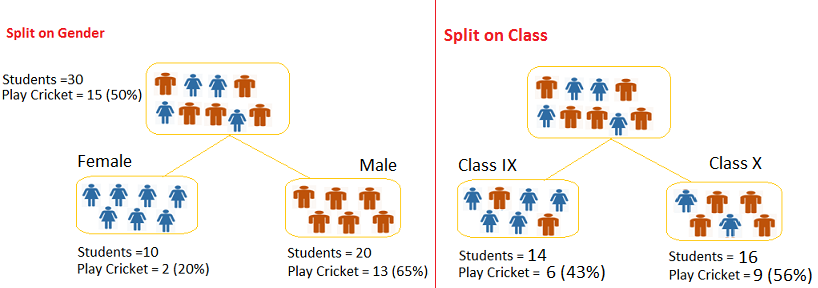
\includegraphics[width=0.9\columnwidth]{./pic/class.png}
\caption{classification samples}
\end{figure}

Split on Gender:
\begin{itemize}
\item Calculate, Gini for sub-node Female = (0.2)*(0.2)+(0.8)*(0.8)=0.68
\item Gini for sub-node Male = (0.65)*(0.65)+(0.35)*(0.35)=0.55
\item Calculate weighted Gini for Split Gender = (10/30)*0.68+(20/30)*0.55 = 0.59
\end{itemize}

Similar for Split on Class:

\begin{itemize}
\item Gini for sub-node Class IX = (0.43)*(0.43)+(0.57)*(0.57)=0.51
\item Gini for sub-node Class X = (0.56)*(0.56)+(0.44)*(0.44)=0.51
\item Calculate weighted Gini for Split Class = (14/30)*0.51+(16/30)*0.51 = 0.51
\end{itemize}

Above, you can see that Gini score for Split on Gender is higher than Split on Class, hence, the node split will take place on Gender.


%---------------------------------------

\item{\textbf{\color{blue} What is Chi-square? How can we use it to design decision tree?}}

It is an algorithm to find out the statistical significance between the differences between sub-nodes and parent node. We measure it by sum of squares of standardized differences between observed and expected frequencies of target variable.

\begin{itemize}
\item It works with categorical target variable “Success” or “Failure”.
\item  It can perform two or more splits.
\item  Higher the value of Chi-Square higher the statistical significance of differences between sub-node and Parent node.
\item  Chi-Square of each node is calculated using formula,
  \bea
\chi^{2} =  \left [ \frac{ (X - E)^2}{E}\right ]^{1/2}
\eea

\item  It generates tree called CHAID (Chi-square Automatic Interaction Detector)
\end{itemize}


Steps to Calculate Chi-square for a split:

\begin{itemize}
\item Calculate Chi-square for individual node by calculating the deviation for Success and Failure both
\item Calculated Chi-square of Split using Sum of all Chi-square of success and Failure of each node of the split
\end{itemize}

\textbf{Example} 

Split on Gender:

First we are populating for node Female, Populate the actual value for “Play Cricket” and “Not Play Cricket”, here these are 2 and 8 respectively.

Calculate expected value for “Play Cricket” and “Not Play Cricket”, here it would be 5 for both because parent node has probability of 50$\%$ and we have applied same probability on Female count(10).

Calculate deviations by using formula, Actual – Expected. It is for “Play Cricket” (2 – 5 = -3) and for “Not play cricket” ( 8 – 5 = 3).

Calculate Chi-square of node for “Play Cricket” and “Not Play Cricket” using formula with formula,$\chi^{2} =  \left [ \frac{ (X - E)^2}{E}\right ]^{1/2}$. You can refer below table for calculation.

Follow similar steps for calculating Chi-square value for Male node.
Now add all Chi-square values to calculate Chi-square for split Gender.
Decision Tree, Chi-Square

\begin{figure}[H]
\centering
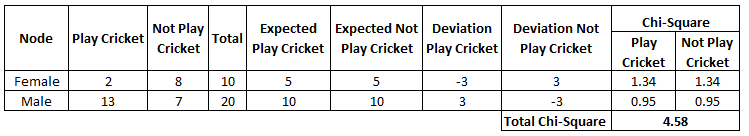
\includegraphics[width=0.9\columnwidth]{./pic/table-1.png}
\caption{classification samples}
\end{figure}


Split on Class:

Perform similar steps of calculation for split on Class and you will come up with below table.

Decision Tree, Chi-SquareAbove, you can see that Chi-square also identify the Gender split is more significant compare to Class.

\begin{figure}[H]
\centering
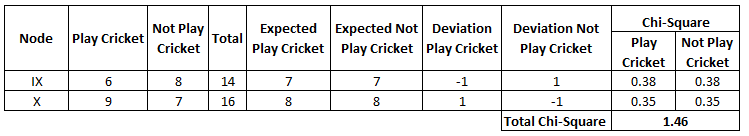
\includegraphics[width=0.9\columnwidth]{./pic/table-2.png}
\caption{classification samples}
\end{figure}



%---------------------------------------

\item{\textbf{\color{blue} What is information gain? How can we use it to design decision tree?}}

https://www.analyticsvidhya.com/blog/2016/04/complete-tutorial-tree-based-modeling-scratch-in-python/

%---------------------------------------


\item{\textbf{\color{blue} What is Reduction in Variance? How can we use it to design decision tree?}}

https://www.analyticsvidhya.com/blog/2016/04/complete-tutorial-tree-based-modeling-scratch-in-python/

%---------------------------------------






\item{\textbf{\color{blue} What do you mean by Greedy Splitting in decision tree? }}

https://machinelearningmastery.com/classification-and-regression-trees-for-machine-learning/


%---------------------------------------

\item{\textbf{\color{blue} How do you set stopping criteria and what is pruning in decision tree? }}

https://machinelearningmastery.com/classification-and-regression-trees-for-machine-learning/

%---------------------------------------













\subsection{Algorithms}

\item{\textbf{\color{blue} What are decision tree algorithm you have heard off?}}
\begin{itemize}

\item ID3 (Iterative Dichotomiser 3) was developed in 1986 by Ross Quinlan. The algorithm creates a multiway tree, finding for each node (i.e. in a greedy manner) the categorical feature that will yield the largest information gain for categorical targets. Trees are grown to their maximum size and then a pruning step is usually applied to improve the ability of the tree to generalise to unseen data.


\item C4.5 is the successor to ID3 and removed the restriction that features must be categorical by dynamically defining a discrete attribute (based on numerical variables) that partitions the continuous attribute value into a discrete set of intervals. C4.5 converts the trained trees (i.e. the output of the ID3 algorithm) into sets of if-then rules. These accuracy of each rule is then evaluated to determine the order in which they should be applied. Pruning is done by removing a rule’s precondition if the accuracy of the rule improves without it.


\item C5.0 is Quinlan’s latest version release under a proprietary license. It uses less memory and builds smaller rulesets than C4.5 while being more accurate.


\item CART (Classification and Regression Trees) is very similar to C4.5, but it differs in that it supports numerical target variables (regression) and does not compute rule sets. CART constructs binary trees using the feature and threshold that yield the largest information gain at each node.
scikit-learn uses an optimised version of the CART algorithm.

\end{itemize}


%-----------------------------------------------------------


\item{\textbf{\color{blue}  What are decision tree classification criteria ?}}  

If a target is a classification outcome taking on values $0,1,…,K-1,$ for node $m$, representing a region $R_m$ with $N_m$ observations, let

\bea
p_{mk} = 1/ N_m \sum_{x_i \in R_m} I(y_i = k)
\eea

be the proportion of class $k$ observations in node $m$
Common measures of impurity are 
1. Gini
\bea
H(X_m) = \sum_k p_{mk} (1 - p_{mk})
\eea
2. Cross-Entropy
\bea
H(X_m) = - \sum_k p_{mk} \log(p_{mk})
\eea
3. Misclassification
\bea
H(X_m) = 1 - \max(p_{mk})
\eea
where $X_m$ is the training data in node $m$

%-----------------------------------------------------------


\item{\textbf{\color{blue}  What are decision tree classification criteria ?}} 

If the target is a continuous value, then for node m, representing a region $R_m$ with $N_m$ observations, common criteria to minimise as for determining locations for future splits are Mean Squared Error, which minimizes the $L2$ error using mean values at terminal nodes, and Mean Absolute Error, which minimizes the $L1$ error using median values at terminal nodes.

1. Mean Squared Error:

\bea
c_m = \frac{1}{N_m} \sum_{i \in N_m} y_i\cr
H(X_m) = \frac{1}{N_m} \sum_{i \in N_m} (y_i - c_m)^2
\eea

2. Mean Absolute Error:
\bea
\bar{y_m} = \frac{1}{N_m} \sum_{i \in N_m} y_i
H(X_m) = \frac{1}{N_m} \sum_{i \in N_m} |y_i - \bar{y_m}|
\eea


\item{\textbf{\color{blue} 30 Questions to test a data scientist on Tree Based Models.}}

\href{https://www.analyticsvidhya.com/blog/2017/09/30-questions-test-tree-based-models/}{30 Questions to test a data scientist on Tree Based Models}


%================================================



\end{enumerate}

\subsection{References}
1. https://www.analyticsvidhya.com/blog/2016/04/complete-tutorial-tree-based-modeling-scratch-in-python/





\begin{itemize}
\item 
\end{itemize}